\documentclass[12pt,a4paper]{article}

% ===== PAKETE =====
\usepackage[ngerman]{babel}          % Deutsche Sprache
\usepackage[utf8]{inputenc}          % UTF-8 Kodierung
\usepackage[T1]{fontenc}             % Schriftkodierung
\usepackage{lmodern}                 % Schönere Schrift
\usepackage[left=2.5cm,right=2.5cm,top=2.5cm,bottom=2.5cm]{geometry}

% Layout & Formatierung
\usepackage{setspace}                % Zeilenabstand


\usepackage{parskip}                 % Absatzformatierung
\usepackage{fancyhdr}                % Kopf- und Fußzeilen

% Bilder & Grafiken
\usepackage{graphicx}                % Bilder einbinden
\usepackage{float}                   % Bessere Positionierung
\usepackage{caption}                 % Bildunterschriften

% Tabellen
\usepackage{tabularx}                % Flexible Tabellen
\usepackage{booktabs}                % Schönere Tabellen

% PDF einbinden
\usepackage{pdfpages}                % Für Deckblatt

% Mathematik (falls benötigt)
\usepackage{amsmath}
\usepackage{amssymb}
\usepackage{siunitx}

% Links & Verweise
\usepackage{hyperref}                % Klickbare Links
\hypersetup{
    colorlinks=true,
    linkcolor=black,
    citecolor=black,
    urlcolor=blue,
    pdftitle={Titel deiner Arbeit},
    pdfauthor={Dein Name}
}

% Literaturverzeichnis
\usepackage[backend=biber,style=numeric,sorting=nty]{biblatex}
\addbibresource{literatur.bib}

% ===== EINSTELLUNGEN =====
\onehalfspacing                      % 1,5-facher Zeilenabstand
\setlength{\parindent}{0pt}          % Keine Einrückung
\pagenumbering{arabic}

% Kopf- und Fußzeilen
\pagestyle{fancy}
\fancyhf{}
\fancyhead[L]{\leftmark}
\fancyhead[R]{\thepage}
\renewcommand{\headrulewidth}{0.4pt}

% ===== DOKUMENT =====
\begin{document}

% Vorgegebenes Deckblatt einbinden
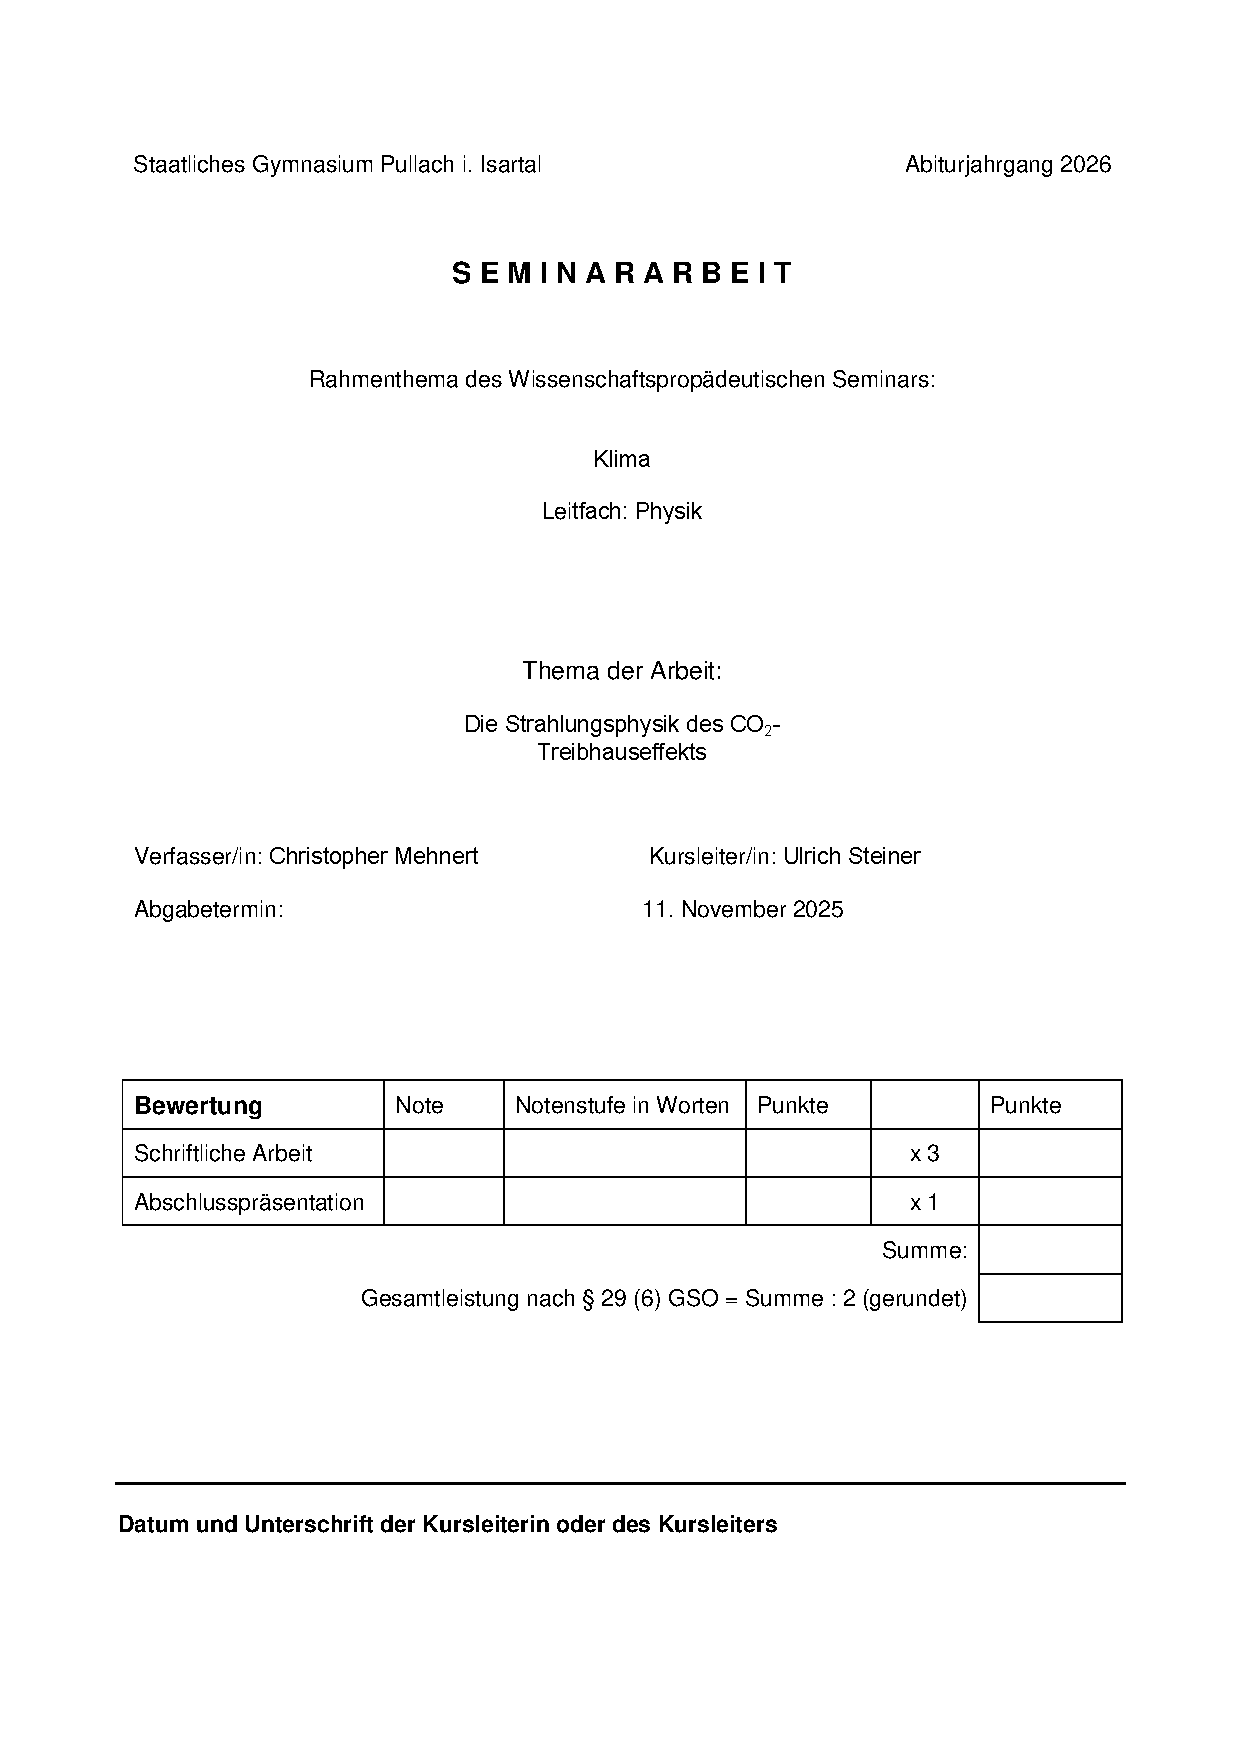
\includepdf[pages={1,2,3}]{assets/deckblatt.pdf}


% Inhaltsverzeichnis
\setcounter{page}{2}
\tableofcontents
\newpage

% Optional: Abbildungsverzeichnis
% \listoffigures
% \newpage

% Optional: Tabellenverzeichnis
% \listoftables
% \newpage

% ===== HAUPTTEIL =====

\section{Einleitung}

\section{Physikalische Grundlagen der Wärmestrahlung}

\subsection{Strahlungsgesetze}
Jedes Medium emittiert elektromagnetische Strahlung zufällig in alle Richtungen. 
Die Intensität dieser Emission hängt sowohl von der Temperatur als auch von den Materialeigenschaften des Mediums ab. 
Der von einer Oberfläche abgegebene Strahlungswärmestrom wird als \textit{spezifische Ausstrahlung} bezeichnet.

Dabei wird zwischen der \textit{gesamten spezifischen Ausstrahlung} $E$ und der \textit{spektralen spezifischen Ausstrahlung} $E_f$ unterschieden:
\begin{align*}
E_f &\equiv \text{abgestrahlte Energie pro Zeit, Oberfläche und Frequenz.} \\
E &\equiv \text{abgestrahlte Energie pro Zeit und Oberfläche.}
\end{align*}
\cite[S.~6--7]{radiativeHeatTransfer}


\subsubsection{Das Plancksche Strahlungsgesetz}

Die spektrale spezifische Ausstrahlung eines ideal schwarzen Körpers wird durch das Plancksche Strahlungsgesetz beschrieben. 
Es gibt an, wie viel Energie pro Zeit, Fläche und Frequenzintervall von einer ideal schwarzen Oberfläche bei einer bestimmten Temperatur $T$ emittiert wird. 
Dieses Gesetz wurde 1900 von Max Planck \cite{plancknormalspektrum}\cite{plancknormalspektrumtheorie} hergeleitet und ist heute als \textit{Plancksches Strahlungsgesetz} bekannt. 
Für eine schwarze Oberfläche, die an ein transparentes Medium mit dem Brechungsindex $n$ grenzt, ergibt sich die spektrale spezifische Ausstrahlung\cite[S.7]{radiativeHeatTransfer} zu:

\begin{equation}
  \label{Plancksche Ausstrahlung Frequenz}
  E_f(T) = \frac{2\pi h f^3 n^2}{c_0^2} \cdot \frac{1}{e^{hf/kT}-1} 
  \quad \text{\cite[S.8]{radiativeHeatTransfer}}
\end{equation}

Angenommen das $n$ über den Wellenlängenbereich konstant ist, lässt sich das Plancksche Strahlungsgesetz auch in Abhängigkeit von der Wellenlänge $\lambda$ formulieren:

\begin{equation}
  \label{Plancksche Ausstrahlung Wellenlänge}
  E_{\lambda}(T) = \frac{2\pi h c_0^2}{n^2\lambda^5} \cdot \frac{1}{e^{hc_0/\lambda kT}-1}
  \quad (n = \text{const}) \quad \text{\cite[S.9]{radiativeHeatTransfer}}
\end{equation}

Dabei bezeichnet $h = \SI{6.626e-34}{\joule\second}$ das Plancksche Wirkungsquantum, 
$c_0 = \SI{2.998e8}{\meter\per\second}$ die Lichtgeschwindigkeit im Vakuum 
und $k = \SI{1.381e-23}{\joule\per\kelvin}$ die Boltzmann-Konstante \cite{codata2018}.

\subsubsection{Das Stefan-Boltzmann Gesetz}
Eine Ober


\subsection{Anwendung auf das System Sonne-Erde}

\section{Molekülphysik des CO\textsubscript{2}}

\subsection{Molekülstruktur und Schwingungsmoden}

\subsection{Quantenmechanische Grundlagen der Absorption}

\subsection{Das CO\textsubscript{2}-Absorptionsspektrum}

\section{Der Treibhauseffekt}

\subsection{Strahlungsbilanz der Erde ohne Atmosphäre}

% ===== LITERATURVERZEICHNIS =====
\newpage
\section{Anhang}

\subsection{Literaturverzeichnis}
\printbibliography[heading=none]

% ===== ANHANG (optional) =====
% \newpage
% \appendix
% \section{Zusätzliche Daten}
% ...

\end{document}